% Gemini theme
% See: https://rev.cs.uchicago.edu/k4rtik/gemini-uccs
% A fork of https://github.com/anishathalye/gemini

\documentclass[final]{beamer}

% ====================
% Packages
% ====================
\usepackage{amsfonts}
\usepackage[T1]{fontenc}
\usepackage{lmodern}
\usepackage[size=custom,width=30,height=36,scale=1.0]{beamerposter}
\geometry{paperwidth=30in,paperheight=36in}
\usetheme{gemini}
\usecolortheme{ucf}
\usepackage{graphicx}
\usepackage{booktabs}
\usepackage{tikz}
\usepackage{pgfplots}
\pgfplotsset{compat=1.17}

% ====================
% Lengths
% ====================

% If you have N columns, choose \sepwidth and \colwidth such that
% (N+1)*\sepwidth + N*\colwidth = \paperwidth
\newlength{\sepwidth}
\newlength{\colwidth}
\setlength{\sepwidth}{0.025\paperwidth}
\setlength{\colwidth}{0.3\paperwidth}

\newcommand{\separatorcolumn}{\begin{column}{\sepwidth}\end{column}}

% ====================
% Title
% ====================

\title{\textbf{DIP Poster Presentation}\\
``Demosaicing of Images''}

\author{Divik Mewari}

\institute[IIITN]{\textit{Indian Institute of Information Technology, Nagpur}}

% ====================
% Footer (optional)
% ====================


\footercontent{
  \href{https://iiitn.ac.in}{https://iiitn.ac.in} \hfill
 Department of ECE, October 2023 \hfill
  \href{mailto:bt20ece041@iiitn.ac.in}{bt20ece041@iiitn.ac.in}}
\begin{document}
\addtobeamertemplate{headline}{}
{
    \begin{tikzpicture}[remember picture,overlay]
      \node [anchor=north west, inner sep=3cm] at ([xshift=0.0cm,yshift=3cm]current page.north west)
      {
\includegraphics[height=11cm]{logos/ucf_logo2.png}}; % also try shield-white.eps
      \node [anchor=north east, inner sep=3cm] at ([xshift=1.0cm,yshift=3cm]current page.north east)
 {
\includegraphics[height=11cm]{logos/YAY.png}};
    \end{tikzpicture}
}

\begin{frame}[t]
\begin{columns}[t]
\separatorcolumn

\begin{column}{\colwidth}

  \begin{block}{Abstract}
  
 Image demosaicing is the process of reconstruction of full color image on the basis of various methods from the data samples obtained by acquisition devices. There are various techniques that can be utilized to achieve demosaiced image by suitably classifying it into various categories.
 \end{block}

  \begin{block}{Introduction}

A demosaicing (also de-mosaicing, demosaicking or debayering) algorithm is a digital image process used to reconstruct a full color image from the incomplete color samples output from an image sensor overlaid with a color filter array (CFA). It is also known as CFA interpolation or color reconstruction. Most modern digital cameras acquire images using a single image sensor overlaid with a CFA, so demosaicing is part of the processing pipeline required to render these images into a viewable format.

\lipsum

\lipsum


\par  Color Filter Array (CFA) interpolation is an indispensable part of image pipeline which is used to recover full resolution image from its CFA data. A CFA is a mosaic of color filters in front of the image sensor. Commercially, the most commonly used CFA configuration is the Bayer filter illustrated here. This has alternating red (R) and green (G) filters for odd rows and alternating green (G) and blue (B) filters for even rows. There are twice as many green filters as red or blue ones, catering to the human eye's higher sensitivity to green light.
\\
\lipsum
\begin{figure}
    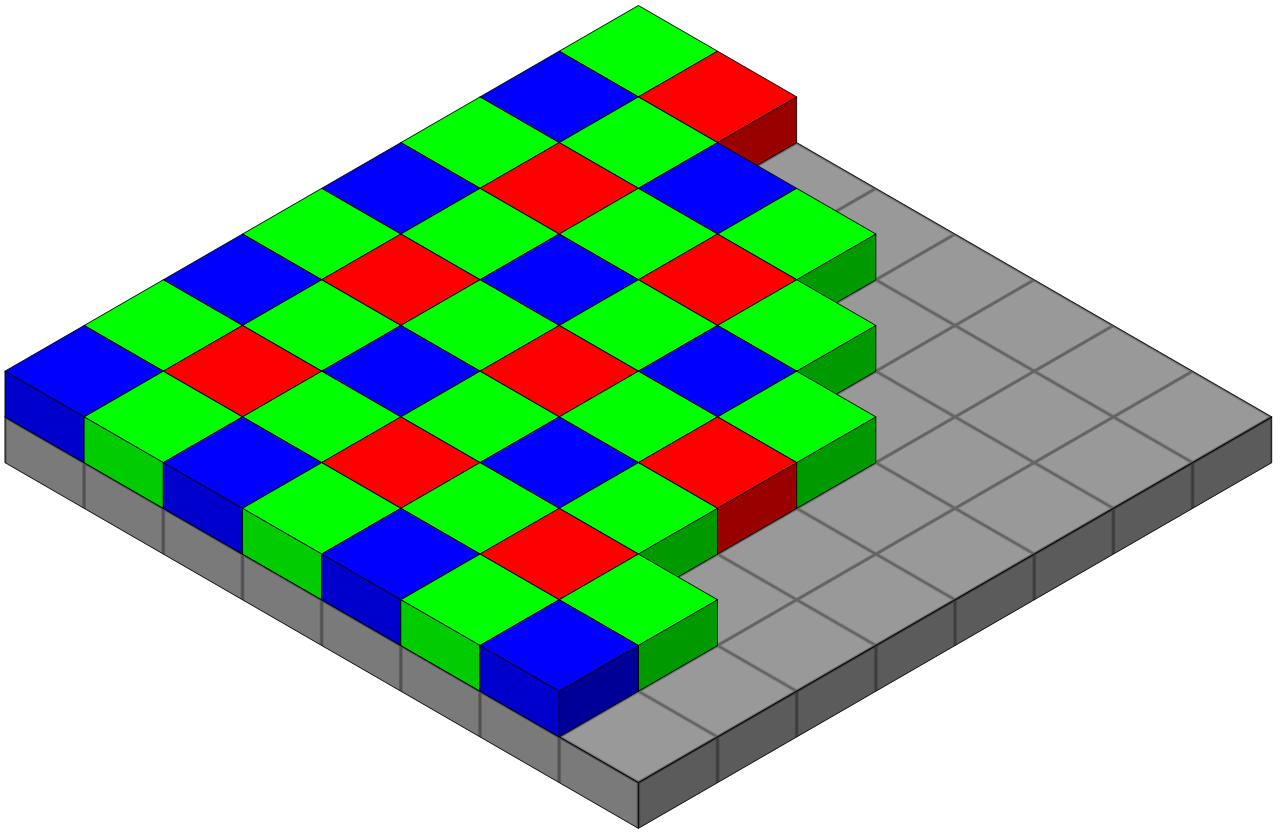
\includegraphics[width=0.8\textwidth]{logos/1280px-Bayer_pattern_on_sensor.svg.png}
\end{figure}

\par The Bayer arrangement of color filters on the pixel array of an image sensor. Each two-by-two cell contains two green, one blue, and one red filter.
Since the color subsampling of a CFA by its nature results in aliasing, an optical anti-aliasing filter is typically placed in the optical path between the image sensor and the lens to reduce the false color artifacts (chromatic aliases) introduced by interpolation.

Since each pixel of the sensor is behind a color filter, the output is an array of pixel values, each indicating a raw intensity of one of the three filter colors. Thus, an algorithm is needed to estimate for each pixel the color levels for all color components, rather than a single component.
\lipsum
\\
  \end{block}
  \begin{figure*}
    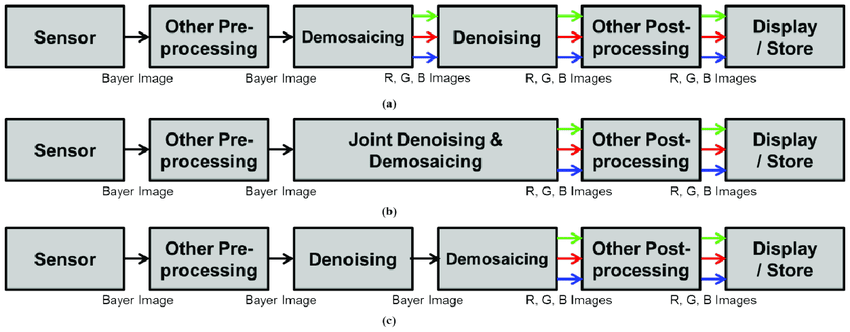
\includegraphics[width=2.0\textwidth]{logos/dip.png}
    \end{figure*}
\end{column}
\separatorcolumn

\begin{column}{\colwidth}

\begin{block}{Image Demosaicing Methods}
  
The plethora of image demosaicing approaches are available but they are broadly classified into six categories as
depicted in Figure 1.
\begin{figure}
    \centering
    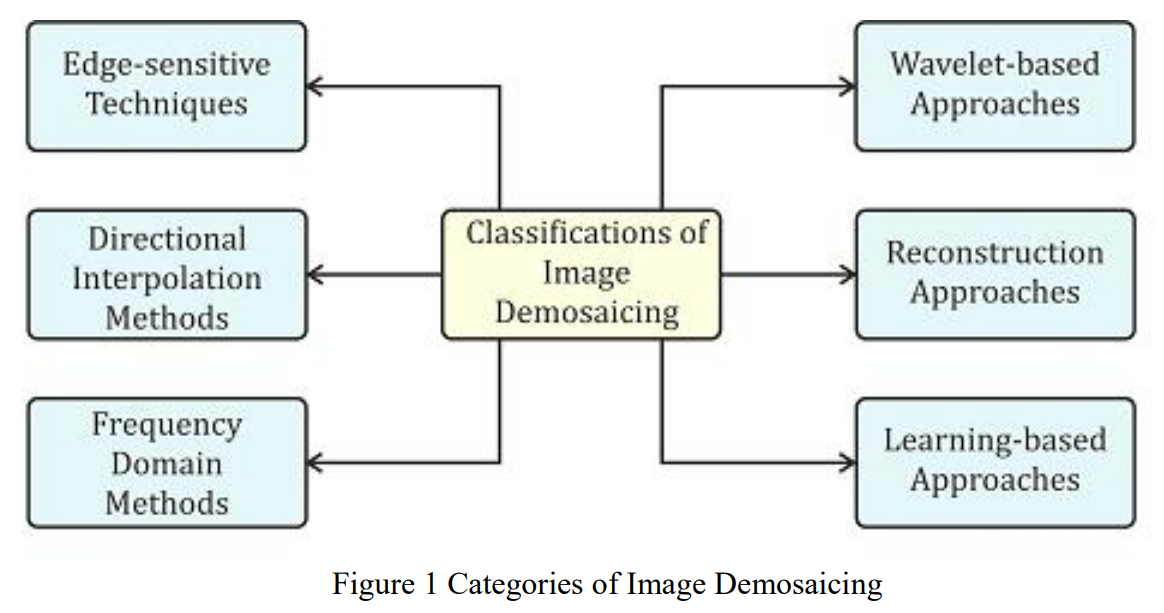
\includegraphics[width=0.9\textwidth]{logos/Screenshot (160).png}
    \label{fig:img1}
\end{figure}
    \par 1. Edge Sensitive Techniques - 
\par - Binary and Adaptive Interpolation \\ - Laplacian operator based adaptive color plane interpolation \\ - Computation of edge slope and false color measure \\ - Median filter and spatial deinterlacing \\ - Heuristic algorithm \\ - Jacobian matrix and neighborhood voting based adaptive demosaicing method 

\begin{figure}
    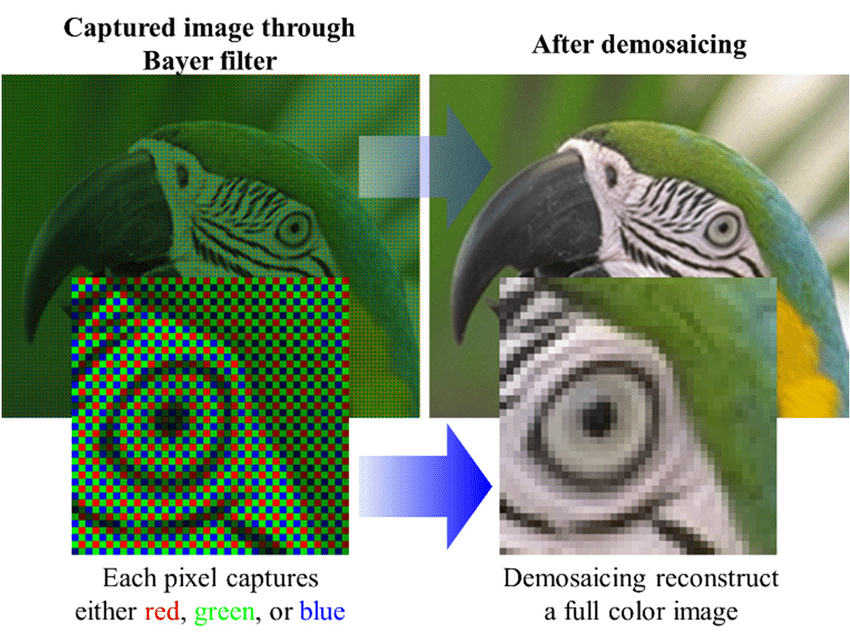
\includegraphics[width=0.8\textwidth]{logos/An-example-of-the-demosaicing-process.png}
    \end{figure}
    
\par 2. Directional Interpolation Techniques - 

\par - FIR filter in horizontal and vertical directions \\ - Spectral-spatial
correlation concept \\ - Cubic spline interpolation \\ - Adaptive thresholding \\ - Chromatic smoothness \\ -  Residual interpolation 

\par 3. Frequency domain methods -
\par - Spatial frequency filtering \\ - Complementary asymmetric filters \\ - Luminance–chrominance based demosaicing algorithm \\ -  Least-squares method for
bandpass filters \\ - Multi-objective optimization technique



\end{block}

\end{column}

\separatorcolumn

\begin{column}{\colwidth}
  
  
\par 4. Wavelet-based approaches - 
\par (Some of the demosaicing employed Discrete Wavelet Transform (DWT) based on low pass and high pass filters for decomposing an image into four subbands, that is, LL, LH, HL, and HH.)
\par - Projections Onto Convex Sets (POCS) approach  \\ - Directional
filtering based approach \\ - Mallat wavelet packet transform \\ -  Gaussian Scale Mixture (GSM) approach \\ - Bayesian minimum mean square error estimation

\par 5. Reconstruction approaches - 

\par - Optimum reconstruction algorithms based on Bayesian method \\ -  Markov Random Field (MRF) \\ - Linear Least Mean Squared Error (LLMSE) \\ - Minimum Mean Square Error (MMSE) based estimator \\ - Unified approach based on posteriori estimation

\par 6.  Learning based methods -
\par (Moreover, learning based techniques is also used in the image demosaicing from previous few years.)
\par - Demosaicing operation by using a sparse model \\ - Convolutional Neural Network (CNN) \\ - Machine learning and deep residual network \\ - Generative Adversarial Network (GAN) 
\vspace{1cm}
 \begin{block}{Applications of Demosaicing}
\begin{enumerate}
    \item The process of image demosaicing can be utilized in the various image processing applications such as in low light images, image forensics, polarization images, medical imaging, hardware platforms.
    \item Further, the demosaicing techniques are also utilized for the application of image forensics, for instance,
demosaicing artifacts can be used for the detection of forged images by analyzing these CFA artifacts.
\item Image demosaicing is also employed in the field of medical imaging that is one of the most important
issues as compressed data in medical images can result in life-threatening conditions. 
\end{enumerate}





  \end{block}
  

\begin{block}{Conclusions}
\par The image demosaicing techniques based on various categories are explored. Further, learning based techniques are used for demosaicing in the recent work that provided promising results as compared to the traditional methods. Since, demosaicing often face the challenge of reducing the zipping and color artifacts. Hence, most of the techniques are aimed to reduce these artifacts for improving its performance. Additionally, demosaicing is also used in combination with denoising and super resolution by some of the techniques. Thus, unified algorithms can be used for performing multiple tasks with reduced complexity. 

\end{block}

\begin{block}{References}
\par 1. Boulos, M. N. K., Wheeler, S., Tavares, C., & Jones, R. (2011). How smartphones are changing the face of
mobile and participatory healthcare: an overview, with example from eCAALYX. Biomedical engineering
online, 10(1), 1-14. \\
2. Kaur, K., Kaur, G., & Kaur, J. (2017). Extraction of Abnormal Portion of Brain Using Jaya Algorithm.
In Proceedings of Sixth International Conference on Soft Computing for Problem Solving (pp. 163-169).
Springer, Singapore.\\
3. Kaur, D., &Walia, G. K. (2020). A Hybrid ACO-SVM Approach for Detecting and Classifying Malaria
Parasites. In Computational Network Application Tools for Performance Management (pp. 139-152).
Springer, Singapore.

 

\end{block}

\end{column}

\separatorcolumn
\end{columns}
\end{frame}

\end{document}
